\documentclass[semifinal]{cpecmu}

%% This is a sample document demonstrating how to use the CPECMU
%% project template. If you are having trouble, see "cpecmu.pdf" for
%% documentation.

\projectNo{69}
\acadyear{2020}

\titleTH{โครงงานสุดเลิฟของฉัน}
\titleEN{Your Project Name Goes Here}

\author{นายกินรี ไทร์ล้ำเลิศ}{Kinnaree Tirelumlert}{690610696}
\author{นายบรรจบ พบเอฟตลอด}{Banjob Pob-eftalord}{690610969}

\cpeadvisor{chinawat}
\cpecommittee{paskorn}
\committee{รศ.ดร.\,นิพนธ์ ธีรอำพน}{Assoc.\,Prof.\,Nipon Theera-Umpon, Ph.D.}

%% Some possible packages to include:
\usepackage[final]{graphicx} % for including graphics

%% Add bookmarks and hyperlinks in the document.
\PassOptionsToPackage{hyphens}{url}
\usepackage[colorlinks=true,allcolors=Blue4,citecolor=red,linktoc=all]{hyperref}
\def\UrlFont{\thaifonttt}

%% Needed just by this example, but maybe not by most reports
\usepackage{afterpage} % for outputting
\usepackage{pdflscape} % for landscape figures and tables. 

%% Some other useful packages. Look these up to find out how to use
%% them.
% \usepackage{natbib}    % for author-year citation styles
% \usepackage{txfonts}
% \usepackage{appendix}  % for appendices on a per-chapter basis
% \usepackage{xtab}      % for tables that go over multiple pages
% \usepackage{subfigure} % for subfigures within a figure
% \usepackage{pstricks,pdftricks} % for access to special PostScript and PDF commands
% \usepackage{nomencl}   % if you have a list of abbreviations

%% if you're having problems with overfull boxes, you may need to increase
%% the tolerance to 9999
% \tolerance=9999

\bibliographystyle{plain}
% \bibliographystyle{IEEEbib}

% \renewcommand{\topfraction}{0.85}
% \renewcommand{\textfraction}{0.1}
% \renewcommand{\floatpagefraction}{0.75}

%% Example for glossary entry
%% Need to use glossary option
%% See glossaries package for complete documentation.
\ifglossary
  \newglossaryentry{lorem ipsum}{
    name=lorem ipsum,
    description={derived from Latin dolorem ipsum, translated as ``pain itself''}
  }
\fi

%% Uncomment this command to preview only specified LaTeX file(s)
%% imported with \include command below.
%% Any other file imported via \include but not specified here will not
%% be previewed.
%% Useful if your report is large, as you might not want to build
%% the entire file when editing a certain part of your report.
% \includeonly{chapters/intro,chapters/background}

\begin{document}
\maketitle
\makesignature

\ifproject
\begin{abstractTH}
% เขียนบทคัดย่อของโครงงานที่นี่
% แพลตฟอร์มนี้ถูกพัฒนาขึ้นเพื่อรวบรวมและจัดเก็บข้อมูลโครงงานวิศวกรรมศาสตร์ของนักศึกษามหาวิทยาลัยเชียงใหม่ โดยมีวัตถุประสงค์หลักในการสร้างแหล่งข้อมูลกลางที่เป็นระบบและเข้าถึงได้ง่าย นักศึกษาสามารถค้นหาและศึกษาโครงงานของรุ่นพี่ เพื่อนำไปเป็นแนวทางหรือแรงบันดาลใจในการพัฒนาโครงงานของตนเอง ระบบถูกออกแบบให้มีการจัดหมวดหมู่และฟังก์ชันการค้นหาที่มีประสิทธิภาพ เพื่อให้การเข้าถึงข้อมูลเป็นไปอย่างสะดวกและรวดเร็ว แพลตฟอร์มนี้จึงเป็นเครื่องมือสำคัญในการสนับสนุนการเรียนรู้และการพัฒนานวัตกรรมของนักศึกษาวิศวกรรมศาสตร์

แพลตฟอร์มนี้ถูกพัฒนาขึ้นโดยมีจุดประสงค์หลักเพื่อเก็บรวบรวมโครงงานวิศวกรรม
ของนักศึกษาคณะวิศวกรรมศาสตร์มหาวิทยาลัยเชียงใหม่ และใช้ในการสร้างแหล่งข้อมูลกลางที่เป็นระบบและเข้าถึงได้ง่าย
\enskip นักศึกษาสามารถค้นหาและศึกษาโครงงานของรุ่นพี่ เพื่อนำไปใช้เป็นแรงบันดาลใจหรือตัวอย่างในการทำโครงงาน \enskip
โดยระบบได้ออกแบบให้สามารถค้นหาได้จากหมวดหมู่ต่างๆ หรือสามารถค้นหาโครงงานที่เกี่ยวห้องได้โดยต้นหาจาก keyword ที่เกี่ยวข้องใน pdf ของโครงงานนั้นๆ

% การเขียนรายงานเป็นส่วนหนึ่งของการทำโครงงานวิศวกรรมคอมพิวเตอร์
% เพื่อทบทวนทฤษฎีที่เกี่ยวข้อง อธิบายขั้นตอนวิธีแก้ปัญหาเชิงวิศวกรรม และวิเคราะห์และสรุปผลการทดลองอุปกรณ์และระบบต่างๆ
% \enskip อย่างไรก็ดี การสร้างรูปเล่มรายงานให้ถูกรูปแบบนั้นเป็นขั้นตอนที่ยุ่งยาก
% แม้ว่าจะมีต้นแบบสำหรับใช้ในโปรแกรม Microsoft Word แล้วก็ตาม
% แต่นักศึกษาส่วนใหญ่ยังคงค้นพบว่าการใช้งานมีความซับซ้อน และเกิดความผิดพลาดในการจัดรูปแบบ กำหนดเลขหัวข้อ และสร้างสารบัญอยู่
% \enskip ภาควิชาวิศวกรรมคอมพิวเตอร์จึงได้จัดทำต้นแบบรูปเล่มรายงานโดยใช้ระบบจัดเตรียมเอกสาร
% \LaTeX{} เพื่อช่วยให้นักศึกษาเขียนรายงานได้อย่างสะดวกและรวดเร็วมากยิ่งขึ้น
\end{abstractTH}

\begin{abstract}
\hspace{1.27cm}This platform was developed with the main purpose of collecting engineering projects of students of the Faculty of Engineering, Chiang Mai University, and used to create a centralized and easily accessible source of information.
\enskip Students can search for and study the projects of their seniors to use as inspiration or examples for doing projects. \enskip
The system is designed to be searchable by various categories or to search for projects related to the room by searching for relevant keywords in the PDF of that project.
\end{abstract}

\iffalse
\begin{dedication}
This document is dedicated to all Chiang Mai University students.

Dedication page is optional.
\end{dedication}
\fi % \iffalse

\begin{acknowledgments}
% Your acknowledgments go here. Make sure it sits inside the
 \hspace{1.27cm}โครงงานนี้จะไม่สามารถสำเร็จได้ถ้าไม่ได้ความกรุณาจาก ผศ. โดม โพธิกานนท์ อาจารย์ที่ปรึกษาโครงงาน ที่ได้สละเวลาให้ความช่วยเหลือให้คำแนะนำและสนับสนุนในการทำโครงงานนี้รวมถึงอ.ดร.ชินวัตร อิศราดิสัยกุล  และ ผศ.ดร.นิรันดร์ พิสุทธอานนท์ ที่ ให้คำปรึกษาจนทำให้โครงงานเล่มนี้เสร็จ
สมบูรณ์ไปได้
% \texttt{acknowledgment} environment.


\acksign{2024}{2}{2}
\end{acknowledgments}%
\fi % \ifproject

\contentspage

\ifproject
\figurelistpage

\tablelistpage
\fi % \ifproject

% \abbrlist % this page is optional

% \symlist % this page is optional

% \preface % this section is optional


\pagestyle{empty}\cleardoublepage
\normalspacing \setcounter{page}{1} \pagenumbering{arabic} \pagestyle{cpecmu}

\chapter{\ifcpe บทนำ\else Introduction\fi}

\section{\ifcpe ที่มาของโครงงาน\else Project rationale\fi}

\section{\ifcpe วัตถุประสงค์ของโครงงาน\else Objectives\fi}
\begin{enumerate}
    \item
\end{enumerate}

\section{\ifcpe ขอบเขตของโครงงาน\else Project scope\fi}

\subsection{\ifcpe ขอบเขตด้านฮาร์ดแวร์\else Hardware scope\fi}

\subsection{\ifcpe ขอบเขตด้านซอฟต์แวร์\else Software scope\fi}

\section{\ifcpe ประโยชน์ที่ได้รับ\else Expected outcomes\fi}

\section{\ifcpe เทคโนโลยีและเครื่องมือที่ใช้\else Technology and tools\fi}

\subsection{\ifcpe เทคโนโลยีด้านฮาร์ดแวร์\else Hardware technology\fi}

\subsection{\ifcpe เทคโนโลยีด้านซอฟต์แวร์\else Software technology\fi}

\section{\ifcpe แผนการดำเนินงาน\else Project plan\fi}

\begin{plan}{6}{2020}{2}{2021}
    \planitem{7}{2020}{8}{2020}{ศึกษาค้นคว้า}
    \planitem{8}{2020}{1}{2021}{ชิล}
    \planitem{2}{2021}{2}{2021}{เผา}
    \planitem{12}{2019}{1}{2022}{ทดสอบ}
\end{plan}

\section{\ifcpe บทบาทและความรับผิดชอบ\else Roles and responsibilities\fi}
อธิบายว่าในการทำงาน นศ. มีการกำหนดบทบาทและแบ่งหน้าที่งานอย่างไรในการทำงาน จำเป็นต้องใช้ความรู้ใดในการทำงานบ้าง

\section{\ifcpe%
ผลกระทบด้านสังคม สุขภาพ ความปลอดภัย กฎหมาย และวัฒนธรรม
\else%
Impacts of this project on society, health, safety, legal, and cultural issues
\fi}

แนวทางและโยชน์ในการประยุกต์ใช้งานโครงงานกับงานในด้านอื่นๆ รวมถึงผลกระทบในด้านสังคมและสิ่งแวดล้อมจากการใช้ความรู้ทางวิศวกรรมที่ได้

\chapter{\ifenglish Background Knowledge and Theory\else ทฤษฎีที่เกี่ยวข้อง\fi}

\hspace{1.27cm}การทำโครงงาน เริ่มต้นด้วยการศึกษาค้นคว้า ทฤษฎีที่เกี่ยวข้อง หรือ งานวิจัย/โครงงาน ที่เคยมีผู้นำเสนอไว้แล้ว ซึ่งเนื้อหาในบทนี้ก็จะเกี่ยวกับการอธิบายถึงสิ่งที่เกี่ยวข้องกับโครงงาน เพื่อให้ผู้อ่านเข้าใจเนื้อหาในบทถัดๆ ไปได้ง่ายขึ้น

\section{ระบบฐานข้อมูล (Database System)}
\hspace{1.27cm}ระบบฐานข้อมูล (Database System) หมายถึงโครงสร้างสารสนเทศที่ประกอบด้วย รายละเอียดของข้อมูลที่เกี่ยวข้องกันที่จะนำมาใช้ในระบบต่าง ๆ ร่วมกัน  ซึ่่งผู้ใช้สามารถจัดการกับ
ข้อมูลได้ในลักษณะต่าง ๆ ทั้งเพิ่ม ลบ หรือแก้ไขตลอดจนการเรียกดูข้อมูล ส่วนใหญ่จะเป็นการประยุกต์นำเอาระบบคอมพิวเตอร์เข้ามาช่วยในการจัดการฐานข้อมูล

ระบบฐานข้อมูล มีคำศัพท์ต่างๆที่เกี่ยวข้องดังนี้

\begin{enumerate}
  \hangindent=2em \hangafter=1
  \item เอนทิตี้ (Entity) หมายถึงสิ่งที่เราสนใจจะเก็บข้อมูล เช่น นักศึกษา อาจารย์ วิชาการ หรือห้องเรียน
  \item แอตทริบิวต์ (Attribute) หมายถึงคุณสมบัติของเอนทิตี้ เช่น ชื่อ นามสกุล หรือรหัสนักศึกษา
  \item ความสัมพันธ์ (Relationship) หมายถึงความสัมพันธ์ระหว่างเอนทิตี้ โดยที่เอนทิตี้หนึ่งสามารถมีความสัมพันธ์กับเอนทิตี้อีกเอนทิตี้หนึ่งได้ เช่น นักศึกษาสามารถลงทะเบียนเรียนในหลายวิชา และวิชาใด ๆ ก็สามารถมีนักศึกษาหลายคนลงทะเบียนเรียนได้
  \item คีย์หลัก (Primary Key) หมายถึงคีย์ที่ใช้เพื่อระบุเอนทิตี้นั้น ๆ อย่างชัดเจน และไม่สามารถซ้ำกันได้  
  \item คีย์นอก (Foreign Key) หมายถึงคีย์ที่เป็นคีย์หลักของเอนทิตี้หนึ่ง และเป็นคีย์ที่อยู่ในเอนทิตี้อีกเอนทิตี้หนึ่ง  
\end{enumerate}



\section{ไมโครเซอร์วิส (Microservices)}
\hspace{1.27cm}Microservice\cite{microservice} หรือ Microservice Architecture คือสถาปัตยกรรมการออกแบบ Service หรือก็คือออกแบบซอฟต์แวร์ โดยการที่ในชื่อมีคำว่า Micro นำหน้าอยู่ก็เพราะว่าเป็นการออกแบบที่ทำให้ Service มีขนาดเล็กเพื่อแก้ไขจุดด้อยของสถาปัตยกรรมการออกแบบอื่นๆ 

\subsection{Monolithic VS Microservice}
\hspace{1.27cm}หาก Microservice เป็นการออกแบบ Service ให้มีขนาดเล็ก การจะเทียบให้เห็นภาพชัดเจนที่สุดก็ต้องเทียบกับ Monolithic ที่เป็นระบบที่มีขนาดใหญ่ โดย Monolithic จะเป็นระบบที่มีการทำงานทั้งหมดอยู่ใน Service เดียว
% Subsection 1 text
% \clearpage
\begin{figure}[H] % 'H' forces placement exactly here
% \begin{figure}[ht] % 'ht' means place it approximately here
  \centering
  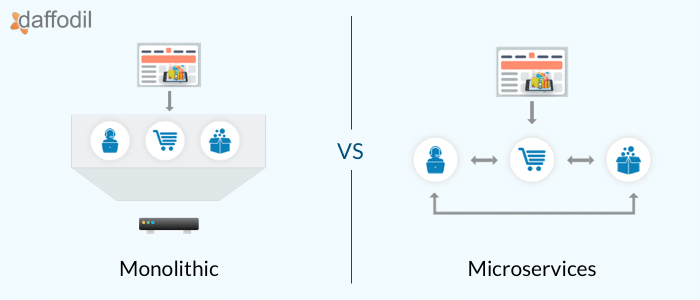
\includegraphics[width=\linewidth, keepaspectratio]{pictures/monolithic-vs-microservices.png}
  \caption[Poem]{รูปจาก nsights.daffodilsw.com}
  % \label{fig:monolithic-vs-microservices}
\end{figure}


\subsubsection{ความแตกต่างระหว่าง Monolithic และ Microservice}
\begin{itemize}
  \item \textbf{Monolithic} เป็นชื่อของสถาปัตยกรรมการออกแบบซอฟต์แวร์หรือ Service ที่มีคนใช้งานเป็นจำนวนมากและมีมาอย่างยาวนาน โดยเป็นลักษณะของระบบที่การทำงานทุกอย่างจะรวมอยู่ในกลุ่มก้อนเดียวกัน และใช้งาน Database เดียวกัน (อย่างในภาพจะเห็นว่าเป็นเว็บไซต์ขายสินค้าที่มีฟังก์ชันจัดการผู้ใช้, ตะกร้าสินค้า และการส่งสินค้า รวมอยู่ด้วยกัน และใช้ฐานข้อมูลเดียวกัน)
  \item \textbf{Microservice}  จะออกแบบโดยแยกการทำงานที่รวมกันเป็นก้อนใหญ่ๆของแบบ Monolithic ออกมาให้เล็กลงโดยอาจจะแยกตามบริการหรือตามฟังก์ชันการทำงานเลยก็ได้ (จากในภาพฟังก์ชันทั้งสามอย่างจะแยกออกจากกัน และไม่ได้ใช้ฐานข้อมูลเดียวกันในการเก็บข้อมูลอีกต่อไป เพราะแต่ละฟังก์ชันหรือบริการที่แยกออกมามีฐานข้อมูลเป็นของตัวเอง และสามารถติดต่อกันได้ผ่าน API )
\end{itemize}




\subsubsection{ข้อดีและข้อเสียของ Microservice}
\begin{itemize}
  \item ข้อดี
  \begin{enumerate}
    \item การทำงานหลักแต่ละส่วนของระบบ ถ้าเป็นไปได้ควรแยกออกเป็น service แต่ละอัน เช่นจัดการสินค้า กับจัดการการซื้อสินค้าก็แยกกันไปเลย
    \item มีที่เก็บข้อมูลของตัวเอง
  \end{enumerate}
  \item ข้อเสีย
  \begin{enumerate}
    \item การจัดการระบบที่มีหลาย service อาจจะทำให้การจัดการระบบทำได้ยากขึ้น
    \item การทำงานของระบบที่แยกออกมาอาจจะทำให้การทำงานของระบบช้าลง
  \end{enumerate}
\end{itemize}
\clearpage
\section{RabbitMQ}
\hspace{1.27cm}RabbitMQ \cite{rabbitmq}ซอฟต์แวร์ที่เป็นตัวกลางรับส่งข้อความระหว่างแอปพลิเคชันต่างๆ ผู้ไปรับรับข้อความจากผู้ส่ง (แอปพลิเคชันหนึ่ง) เก็บไว้รอการคัดแยก และส่งต่อให้ผู้รับ (แอปพลิเคชันอีกแอปพลิเคชันหนึ่ง) เหมาะสำหรับการทำแอปพลิเคชันที่ต้องมีการจัดคิวในการส่งข้อความ ระบบที่เป็นไมโครเซอร์วิสเอาไว้สื่อสารกันได้อย่างมีประสิทธิภาพ ทำให้สามารถแบ่งงานขนาดใหญ่เป็นงานย่อยๆ และส่งไปยังระบบอื่นๆ เพื่อประมวลผลได้นั่นเอง
\begin{figure}[H] % 'H' forces placement exactly here
  % \begin{figure}[ht] % 'ht' means place it approximately here
    \centering
    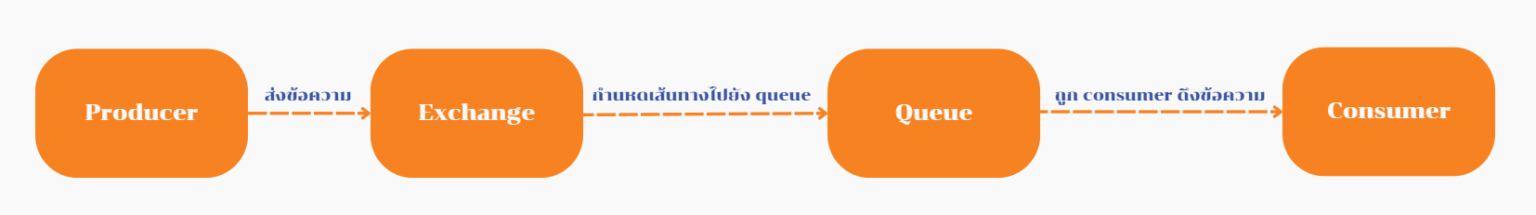
\includegraphics[width=\linewidth, keepaspectratio]{pictures/rabbitmq.png}
    \caption[Poem]{รูปจาก https://www.borntodev.com/2024/06/09/rabbitmq-nodejs/}
    \label{fig:rabbitmq}
\end{figure}
  \subsection{คำศัพท์ต่างๆที่เกี่ยวข้อง}
  \begin{itemize}
    \item \textbf{Producer} คือ ผู้ส่งข้อความ
    \item \textbf{Consumer} คือ ผู้รับข้อความ
    \item \textbf{Queue} คือ คิวข้อความ
    \item \textbf{Exchange} คือ ตัวกลางในการส่งข้อความ
    \item \textbf{Binding} คือ การเชื่อมต่อระหว่าง Exchange กับ Queue
    \item \textbf{Channel} คือ ช่องสื่อสารระหว่าง Producer และ Consumer
    \item \textbf{Connection} คือ การเชื่อมต่อระหว่าง RabbitMQ กับ Producer และ Consumer
  \end{itemize}
% Section 3 text. The dielectric constant\index{dielectric constant}
% at the air-metal interface determines
% the resonance shift\index{resonance shift} as absorption or capture occurs
% is shown in Equation~\eqref{eq:dielectric}:

% \begin{equation}\label{eq:dielectric}
% k_1=\frac{\omega}{c({1/\varepsilon_m + 1/\varepsilon_i})^{1/2}}=k_2=\frac{\omega
% \sin(\theta)\varepsilon_\mathit{air}^{1/2}}{c}
% \end{equation}

% \noindent
% where $\omega$ is the frequency of the plasmon, $c$ is the speed of
% light, $\varepsilon_m$ is the dielectric constant of the metal,
% $\varepsilon_i$ is the dielectric constant of neighboring insulator,
% and $\varepsilon_\mathit{air}$ is the dielectric constant of air.

\section{Framework ที่ใช้ในการพัฒนา}
\hspace{1.27cm}Framework อาจหมายถึง ชุดคำสั่ง เครื่องมือ หรือโครงสร้างอย่างใดอย่างหนึ่ง
ที่สร้างขึ้นมาเพื่ออำนวยความสะดวกแก่ผู้ใช้งาน ซึ่ง Framework มีหลายประเภท หลายแบบ และจะมีวิธีการใช้ที่คล้ายๆกัน
\subsection{Next.js}
\begin{figure}[H] % 'H' forces placement exactly here
  % \begin{figure}[ht] % 'ht' means place it approximately here
    \centering
    
\includegraphics[width=60mm, keepaspectratio ]{pictures/nextjs.png}
    \caption[Poem]{รูปจาก https://medium.com/geekculture/why-should-you-learn-next-js-in-2021-what-are-the-benefits-8292d79bc50c}
    \label{fig:nextjs}
\end{figure}
\hspace{1.27cm}Next.js\cite{Nextjs} คือ JavaScript webapps framework ถูกสร้างขึ้น on top จาก library อย่าง React, Webpack, และ Babel ขึ้นมาอีกที มีจุดเด่นคือ เป็น SSR (server-side rendering) ตั้งแต่ต้น
\subsubsection{ข้อดีของ Next.js}
\begin{itemize}
  \item สามารถทำ SSR ได้ง่าย
  \item มีการจัดการ SEO ที่ดี
  \item Hot reload เวลาเราแก้ไขไฟล์ หน้าเว็บของเราจะถูก refresh โดยอัตโนมัติ 
  \item Project Structure ที่ชัดเจนที่ถูกออกแบบมาให้เรียบร้อยแล้ว
  \item Routing ด้วยความที่มี project structure การทำ routingจึงสามารถ auto routing ได้
\end{itemize}


\subsection{ElysiaJs}
\begin{figure}[H] % 'H' forces placement exactly here
  % \begin{figure}[ht] % 'ht' means place it approximately here
    \centering
    
\includegraphics[width=80mm, keepaspectratio ]{pictures/elysia.jpg}
    \caption[Poem]{รูปจาก https://sadewawicak25.medium.com/file-upload-and-security-validation-on-elysia-js-2-d6c57b023441}
    \label{fig:elysia}
\end{figure}
\hspace{1.27cm}ElysiaJS\cite{ElysiaJs} คือ Framework ในการพัฒนา API ด้วยภาษา Typescript โดยมีจุดเด่นคือ ความเร็วที่เร็วกว่า Express ถึง 21 เท่า (เนื่องจาก ElysiaJS มีการใช้ Bun เป็น Runtime) และอีกจุดเด่นคือ End-to-end Type Safety หรือชนิดของข้อมูลที่ชัดเจน ทำให้เวลาเราทำงานร่วมกับผู้อื่นสามารถทำได้สะดวกมากยิ่งขึ้น เพราะไม่ต้องมาทะเลาะกันเรื่องชนิดของข้อมูลที่ส่งให้กัน อีกทั้งยังมี Community ที่เติบโตเร็ว


\subsection{Gin}
\begin{figure}[H]
  \centering
  
\includegraphics[width=40mm, keepaspectratio ]{pictures/gin.png}
  \caption[Poem]{รูปจาก https://www.askme.co.th/article/what-is-docker/}
  \label{fig:gin}
\end{figure}
\hspace{1.27cm}Gin\cite{Gin101} เป็น web framework ที่เขียนด้วยภาษา golang ที่ถูกพัฒนาต่อมาจาก Martini API ที่หยุดพัฒนาไปแล้ว โดย Gin จะใช้ customized httprouter ทำให้มีประสิทธิภาพด้านความเร็วที่สูงมากกว่า Martini ถึง 40 \cite{GinFeature}เท่า ทำให้มีperformance กับ productivity ที่ดี 

\subsubsection{Feature สำคัญของ Gin มีดังนี้ }
\begin{itemize}
  \item \textbf{JSON validation} สามารถแปลงและตรวจสอบ JSON ของ HTTP request
  \item \textbf{Routes grouping} จัดกลุ่ม routes ของ request ว่า request ไหนต้องมีการ authorization หรือไม่จำเป็นต้องมี การแยก request ด้วย version ของ API โดยสามารถจัดกลุ่มได้อย่างไม่จำกัด และไม่กระทบกับประสิทธิภาพ
  \item \textbf{Middleware support} incoming HTTP request จะถูกจัดการด้วย chain ของ middleware และ action สุดท้าย
  \item \textbf{Rendering build-in} ง่ายสำหรับสร้าง API ที่ render เป็น JSON, XML และ HTML
  \item \textbf{Error management} สามารถจัดการ error ที่เกิดขึ้นในระดับ application และ HTTP ได้
\end{itemize}

\subsection{Docker}
\begin{figure}[H]
  \centering
  
\includegraphics[width=100mm, keepaspectratio ]{pictures/docker.png}
  \caption[Poem]{รูปจาก https://www.docker.com/}
  \label{fig:docker}
\end{figure}

\hspace{1.27cm}Docker เป็นแพลตฟอร์มโอเพนซอร์สที่ช่วยในการสร้าง ทดสอบ และปรับใช้แอปพลิเคชันในรูปแบบของคอนเทนเนอร์ คอนเทนเนอร์เป็นสภาพแวดล้อมที่แยกจากกันที่สามารถรันแอปพลิเคชันได้ โดยที่ไม่ต้องกังวลเกี่ยวกับการกำหนดค่าหรือการติดตั้งซอฟต์แวร์เพิ่มเติมในระบบปฏิบัติการหลักของเซิร์ฟเวอร์ที่ใช้

\hspace{0.8cm}สิ่งที่ทำให้ Docker แตกต่างจากเทคโนโลยีอื่นๆ เช่น Virtual Machines (VMs) คือ Docker ใช้ Kernel ของระบบปฏิบัติการเดียวกันในการรันคอนเทนเนอร์แต่ละตัว ทำให้มีประสิทธิภาพในการใช้งานทรัพยากรสูงขึ้น และทำให้คอนเทนเนอร์ใช้เวลาในการเริ่มต้นที่รวดเร็ว

\subsubsection{องค์ประกอบหลักของ Docker}
\begin{itemize}
  \item \textbf{Docker Engine} เป็นซอฟต์แวร์ที่รันอยู่เบื้องหลังซึ่งทำหน้าที่สร้างและจัดการคอนเทนเนอร์ในระบบ มันมีองค์ประกอบย่อย 2 ส่วนที่สำคัญ ได้แก่
  \begin{enumerate}
    \item Docker Daemon (dockerd): เป็นโปรแกรมหลักที่รันอยู่เบื้องหลังและรับคำสั่งจาก Docker Client ผ่าน API โดย Daemon จะจัดการทุกอย่างที่เกี่ยวข้องกับคอนเทนเนอร์ เช่น การสร้าง, การเริ่มต้น, การหยุด, และการลบคอนเทนเนอร์
    \item Docker CLI (docker): คือส่วนที่ผู้ใช้ใช้ในการสั่งการ Docker ผ่านคำสั่งต่างๆ ผ่าน Command Line Interface เช่น การสร้างคอนเทนเนอร์ (docker run), การสร้างอิมเมจ (docker build), และการจัดการเครือข่าย (docker network)
  \end{enumerate}
  \item \textbf{Docker Image} คือไฟล์แบบคงที่ที่บรรจุโค้ดแอปพลิเคชันและทุกสิ่งที่แอปพลิเคชันนั้นต้องการในการรัน เช่น ไลบรารี, การตั้งค่า, และไฟล์ระบบ Image ถูกสร้างจากไฟล์ที่เรียกว่า Dockerfile ซึ่งเป็นไฟล์ที่กำหนดขั้นตอนในการติดตั้งและตั้งค่าแอปพลิเคชัน
  
  \hspace{1cm}\textbf{Dockerfile Syntax} ที่ใช้ในการสร้าง Image มีคำสั่งที่เป็นลำดับขั้นตอน ยกตัวอย่างเช่น
  \hspace{1cm}\begin{enumerate}
    \item FROM: ระบุ Image เบื้องต้น เช่น Ubuntu, Alpine หรือ Node.js
    \item RUN: รันคำสั่งใน Image เช่น การติดตั้งแพ็คเกจ
    \item COPY/ADD: คัดลอกไฟล์จากโฮสต์เข้าสู่ Image
    \item CMD/ENTRYPOINT: กำหนดคำสั่งที่รันเมื่อคอนเทนเนอร์เริ่มทำงาน
  \end{enumerate}
  \item \textbf{Docker Container} คือ สิ่งที่ถูกสร้างจาก Docker Image และเป็นสภาพแวดล้อมที่แยกจากกันที่สามารถรันแอปพลิเคชันได้โดยมีคุณสมบัติดังนี้
  \item \begin{enumerate}
    \item แยกการทำงานจากระบบปฏิบัติการโฮสต์ แต่ยังใช้เคอร์เนลร่วมกัน
    \item สามารถสร้าง, ลบ, หยุด, และรีสตาร์ทได้อย่างง่ายดาย
    \item สามารถแชร์ทรัพยากรเครือข่ายและไฟล์ระหว่างคอนเทนเนอร์ต่างๆ ได้
  \end{enumerate}
\end{itemize}

\subsubsection{ความแตกต่างระหว่าง Docker กับ Virtual Machines}
\tolerance= 9999
\begin{table}[H]
  \centering
  \caption{เปรียบเทียบคุณสมบัติของ Docker และ Virtual Machine (VM)}
  \label{tab:docker-vm}

  \renewcommand{\arraystretch}{1.3} % Adjust row spacing
  \setlength{\extrarowheight}{3pt}  % Extra row height for better spacing
  \setlength{\tabcolsep}{8pt}       % Adjust column padding

  
  \begin{tabular}{|>{\raggedright\arraybackslash}p{3cm}|>{\raggedright\arraybackslash}p{5cm}|>{\raggedright\arraybackslash}p{5cm}|}
    % Balanced column widths
      \hline
      \rowcolor{gray!20} 
      \textbf{คุณสมบัติ} & \textbf{Docker} & \textbf{Virtual Machine (VM)} \\
      \hline
      การใช้เคอร์เนล & ใช้เคอร์เนลของระบบปฏิบัติการโฮสต์ & จำลองระบบปฏิบัติการเต็มรูปแบบ \\
      \hline
      ขนาดไฟล์ & ขนาดเล็ก & ขนาดใหญ่ \\
      \hline
      เวลาเริ่มต้น & เริ่มต้นได้อย่างรวดเร็ว & ใช้เวลามากขึ้น \\
      \hline
      การใช้ทรัพยากร & ใช้ทรัพยากรน้อย & ใช้ทรัพยากรมาก \\
      \hline
      ความยืดหยุ่น & เหมาะสำหรับแอปพลิเคชันแบบไมโครเซอร์วิส & เหมาะสำหรับการจำลองระบบขนาดใหญ่ \\
      \hline
      การแยกทรัพยากร & แยกการทำงานในระดับแอปพลิเคชัน & แยกระบบปฏิบัติการทั้งหมด \\
      \hline
  \end{tabular}
\end{table}

\hspace{1.27cm}โดยรวมแล้ว Docker เหมาะสำหรับการรันแอปพลิเคชันที่ต้องการความยืดหยุ่นในการปรับใช้และทรัพยากรที่มีข้อจำกัด ในขณะที่ VM เหมาะกับการรันระบบที่ต้องการการแยกสภาพแวดล้อมอย่างสมบูรณ์ เช่น การรันหลายระบบปฏิบัติการในเครื่องเดียวกัน



% define a command that produces some filler text, the lorem ipsum.
% \newcommand{\loremipsum}{
%   \textit{Lorem ipsum dolor sit amet, consectetur adipisicing elit, sed do
%   eiusmod tempor incididunt ut labore et dolore magna aliqua. Ut enim ad
%   minim veniam, quis nostrud exercitation ullamco laboris nisi ut
%   aliquip ex ea commodo consequat. Duis aute irure dolor in
%   reprehenderit in voluptate velit esse cillum dolore eu fugiat nulla
%   pariatur. Excepteur sint occaecat cupidatat non proident, sunt in
%   culpa qui officia deserunt mollit anim id est laborum.}\par}

% \begin{figure}
%   \centering

%   \fbox{
%      \parbox{.6\textwidth}{\loremipsum}
%   }

%   % To include an image in the figure, say myimage.pdf, you could use
%   % the following code. Look up the documentation for the package
%   % graphicx for more information.
%   % \includegraphics[width=\textwidth]{myimage}

%   \caption[Sample figure]{This figure is a sample containing \gls{lorem ipsum},
%   showing you how you can include figures and glossary in your report.
%   You can specify a shorter caption that will appear in the List of Figures.}
%   \label{fig:sample-figure}
% \end{figure}

% Using \verb.\label. and \verb.\ref. commands allows us to refer to
% figures easily. If we can refer to Figures
% \ref{fig:walrus} and \ref{fig:sample-figure} by name in the {\LaTeX}
% source code, then we will not need to update the code that refers to it
% even if the placement or ordering of the figures changes.

% \loremipsum\loremipsum

% This code demonstrates how to get a landscape table or figure. It
% uses the package lscape to turn everything but the page number into
% landscape orientation. Everything should be included within an
% \afterpage{ .... } to avoid causing a page break too early.
% \afterpage{
%   \begin{landscape}
%   \begin{table}
%     \caption{Sample landscape table}
%     \label{tab:sample-table}

%     \centering

%     \begin{tabular}{c||c|c}
%         Year & A & B \\
%         \hline\hline
%         1989 & 12 & 23 \\
%         1990 & 4 & 9 \\
%         1991 & 3 & 6 \\
%     \end{tabular}
%   \end{table}
%   \end{landscape}
% }

% \loremipsum\loremipsum\loremipsum

\section{Overfull hbox}

When the \verb.semifinal. option is passed to the \verb.cpecmu. document class,
any line that is longer than the line width, i.e., an overfull hbox, will be
highlighted with a black solid rule:
\begin{center}
\begin{minipage}{10em}
juxtaposition
\end{minipage}
\end{center}

\section{\ifenglish%
\ifcpe CPE \else ISNE \fi knowledge used, applied, or integrated in this project
\else%
ความรู้ตามหลักสูตรซึ่งถูกนำมาใช้หรือบูรณาการในโครงงาน
\fi
}

อธิบายถึงความรู้ และแนวทางการนำความรู้ต่างๆ ที่ได้เรียนตามหลักสูตร ซึ่งถูกนำมาใช้ในโครงงาน

\section{\ifenglish%
Extracurricular knowledge used, applied, or integrated in this project
\else%
ความรู้นอกหลักสูตรซึ่งถูกนำมาใช้หรือบูรณาการในโครงงาน
\fi
}

อธิบายถึงความรู้ต่างๆ ที่เรียนรู้ด้วยตนเอง และแนวทางการนำความรู้เหล่านั้นมาใช้ในโครงงาน

\chapter{\ifproject%
\ifenglish Project Structure and Methodology\else โครงสร้างและขั้นตอนการทำงาน\fi
\else%
\ifenglish Project Structure\else โครงสร้างของโครงงาน\fi
\fi
}

% ในบทนี้จะกล่าวถึงหลักการ และการออกแบบระบบ

\newcommand{\iptoDomain}[2]{\texttt{#1} $\rightarrow$ \texttt{#2}}

\makeatletter

% \renewcommand\section{\@startsection {section}{1}{\z@}%
%                                    {13.5ex \@plus -1ex \@minus -.2ex}%
%                                    {2.3ex \@plus.2ex}%
%                                    {\normalfont\large\bfseries}}

\makeatother
%\vspace{2ex}
% \titleformat{\section}{\normalfont\bfseries}{\thesection}{1em}{}
% \titlespacing*{\section}{0pt}{10ex}{0pt}

\section{\ifenglish System Architecture\else สถาปัตยกรรมระบบ\fi}

\hspace{1.27cm} \raggedright โครงงานนี้ได้ออกแบบสถาปัตยกรรมของระบบเป็นแบบ Microservices โดยบทนี้จะกล่าวถึงโครงสร้างของระบบทั้งหมด และอธิบายถึงแต่ละส่วนของระบบ โดยระบบจะถูกแบ่งออกเป็นส่วนย่อยๆแต่ละส่วนจะมีหน้าที่และความรับผิดชอบในการทำงานที่แตกต่างกัน 

\begin{figure}[H]
    \centering
    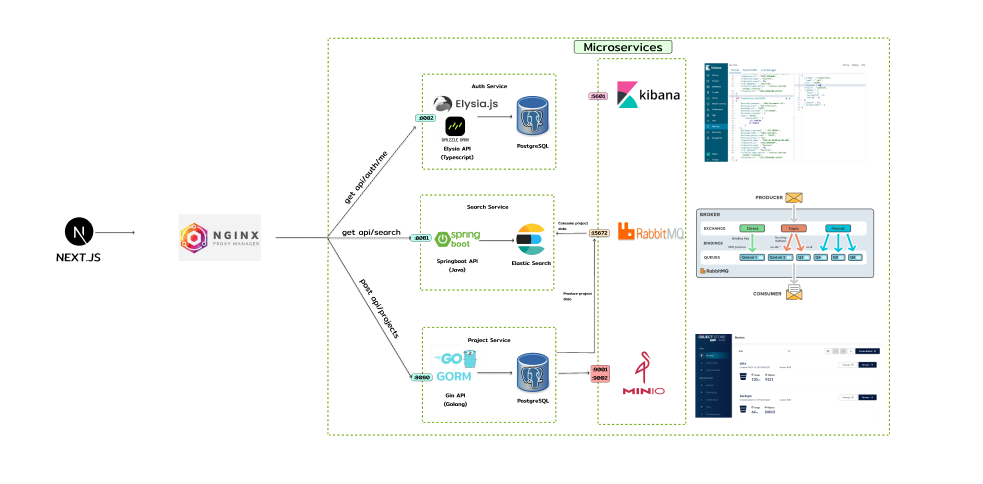
\includegraphics[width=0.8\textwidth]{pictures/architecture.png}
    \caption{รูปภาพแสดงสถาปัตยกรรมของระบบ}
    \label{fig:system_architecture}
  
\end{figure}

จากรูปที่ \ref{fig:system_architecture} แสดงถึงสถาปัตยกรรมของระบบที่ถูกแบ่งออกเป็นส่วนย่อยๆ ดังนี้
\begin{enumerate}
  \item  \textbf{Frontend} ส่วนนี้เป็นส่วนที่ทำหน้าที่ในการแสดงผลของระบบ โดยส่วนนี้จะถูกพัฒนาด้วย Next.js
  \item \textbf{Reverse Proxy} ส่วนนี้เป็นส่วนที่ทำหน้าที่ในการจัดการการเชื่อมต่อระหว่าง Frontend และ Backend โดยส่วนนี้จะถูกพัฒนาด้วย Nginx Proxy Manager(NPM)
  \item \textbf{Backend} ส่วนนี้เป็นส่วนที่ทำหน้าที่ในการจัดการข้อมูลและการทำงานของระบบ โดยส่วนนี้จะถูกแบ่งออกเป็นส่วนย่อยๆ ดังนี้
  \begin{itemize}
    \item \textbf{Auth Service} ส่วนนี้เป็นส่วนที่ทำหน้าที่ในการจัดการข้อมูลของผู้ใช้งาน โดยส่วนนี้จะถูกพัฒนาด้วย Typescript Elysia.js 
    \item \textbf{Project Service} ส่วนนี้เป็นส่วนที่ทำหน้าที่ในการจัดการข้อมูลของโครงงาน โดยส่วนนี้จะถูกพัฒนาด้วย Go Gin 
    \item \textbf{Search Service} ส่วนนี้เป็นส่วนที่ทำหน้าที่ในการค้นหาข้อมูลของโครงงาน โดยส่วนนี้จะถูกพัฒนาด้วย Java Sprint Boot \& Elasticsearch
  \end{itemize}
\end{enumerate}

\section{Frontend (Waiting for edit)}
\hspace{1.27cm} \raggedright ส่วนนี้เป็นส่วนที่ทำหน้าที่ในการแสดงผลของระบบ โดยส่วนนี้จะถูกพัฒนาด้วย Next.js โดยส่วนนี้จะถูกแบ่งออกเป็นส่วนย่อยๆ ดังนี้
\begin{itemize}
  \item \textbf{Home Page} ส่วนนี้เป็นส่วนที่ทำหน้าที่ในการแสดงผลหน้าแรกของเว็บไซต์
  \item \textbf{Project Page} ส่วนนี้เป็นส่วนที่ทำหน้าที่ในการแสดงผลหน้าโครงงาน
  \item \textbf{Search Page} ส่วนนี้เป็นส่วนที่ทำหน้าที่ในการแสดงผลหน้าค้นหา
  \item \textbf{Profile Page} ส่วนนี้เป็นส่วนที่ทำหน้าที่ในการแสดงผลหน้าโปรไฟล์
  \end{itemize}
\section{Reverse Proxy}
\hspace{1.27cm} \raggedright ส่วนนี้เป็นส่วนที่ทำหน้าที่ในการจัดการการเชื่อมต่อระหว่าง Frontend และ Backend โดยส่วนนี้จะถูกพัฒนาด้วย Nginx Proxy Manager(NPM)\cite{npm} มีหน้าที่คือ
การแปลง ip addres ของ server ให้เป็น domain name ยกตัวอย่างเช่น แปลง IP Addres
\iptoDomain{139.59.117.147:8080}{domainname.com}
\enskip โดยส่วนนี้จะทำให้เราสามารถเข้าถึงเว็บไซต์ผ่าน domainname.com ได้ และยังสามารถจัดการการเชื่อมต่อระหว่าง Frontend และ Backend ได้อีกด้วย
\begin{figure}[H]
  \centering
  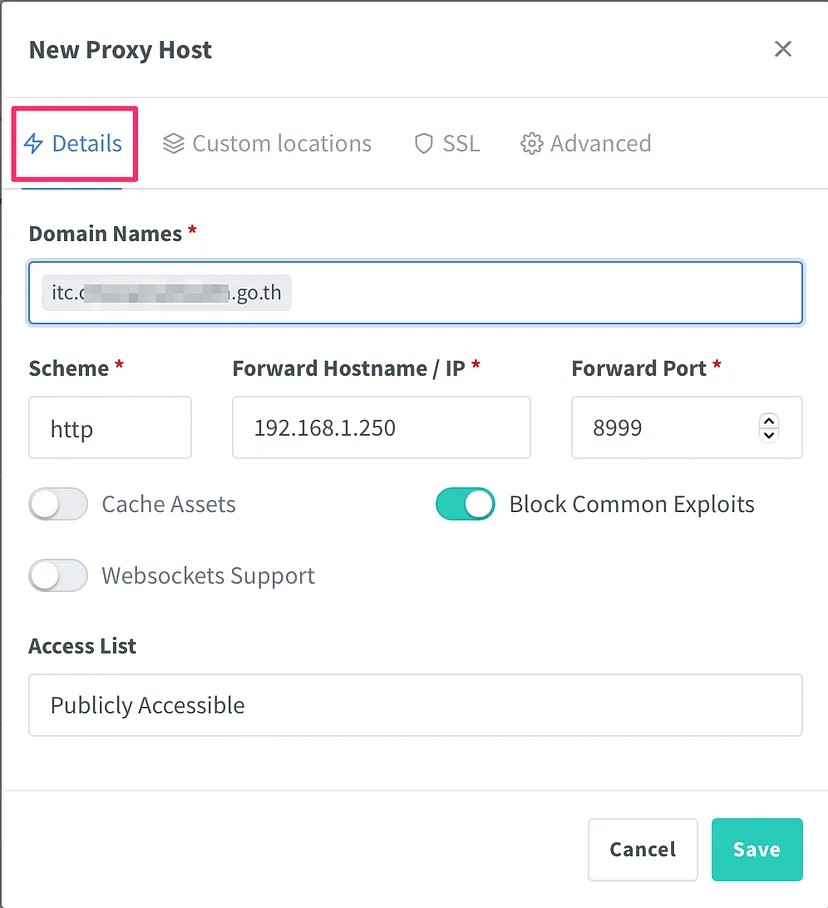
\includegraphics[width=0.8\textwidth]{pictures/npm1.png}
  \caption{รูปภาพแสดงการทแปลง IP ของ Nginx Reverse Proxy}
  \label{fig:reverse_proxy}
\end{figure}
\hspace{ 1.27cm}อีก feature นึงที่สำคัญของ Nginx Reverse Proxy คือการจัดการ SSL Certificate โดย Reverse Proxy จะทำหน้าที่ในการจัดการ SSL Certificate ให้กับเว็บไซต์ ซึ่งจะทำให้เว็บไซต์มีความปลอดภัยมากขึ้น และยังสามารถใช้งานได้ทั้งบน http และ https อีกด้วย
\begin{figure}
  \centering
  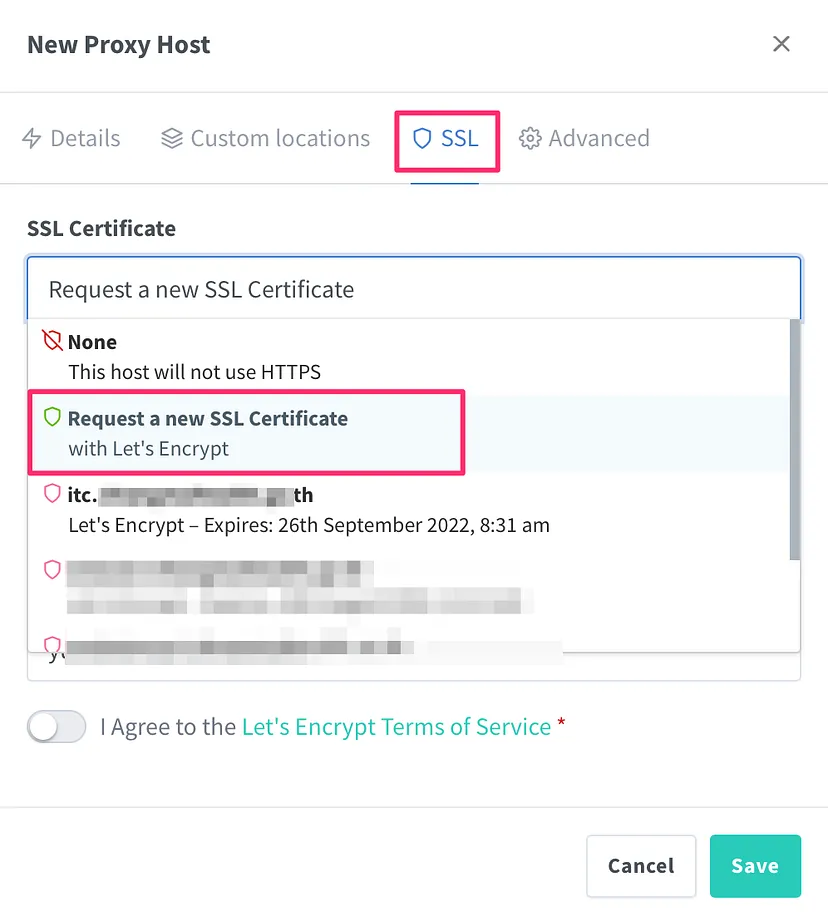
\includegraphics[width=0.8\textwidth]{pictures/encrpt.png}
  \caption{รูปภาพแสดงการจัดการ SSL Certificate ของ Nginx Reverse Proxy}
  \label{fig:reverse_proxy_ssl}
\end{figure}
\section{Backend}
\hspace{1.27cm} \raggedright ส่วนนี้เป็นส่วนที่ทำหน้าที่ในการจัดการข้อมูลและการทำงานของระบบ โดยส่วนนี้จะถูกแบ่งออกเป็นส่วนย่อยๆ ดังนี้
\subsection{Auth Service} 
\hspace{1.27cm} \raggedright ส่วนนี้เป็นส่วนที่ทำหน้าที่ในการจัดการข้อมูลของผู้ใช้งาน โดยส่วนนี้จะถูกพัฒนาด้วย Typescript Elysia.js โดยส่วนนี้จะมีหน้าที่คือ
จัดการข้อมูลของผู้ใช้งานทำหน้าที่ในการเข้าสู่ระบบ และจัดการสิทธิ์ของผู้ใช้งาน(Role) โดยมีการใช้งาน Oauth2 ในการจัดการการเข้าสู่ระบบ และมีการใช้งาน JWT เพื่อสร้าง Token ส่งกลับไปยัง Frontend
\subsubsection{Database Schema}
\begin{figure}[H]
  \centering
  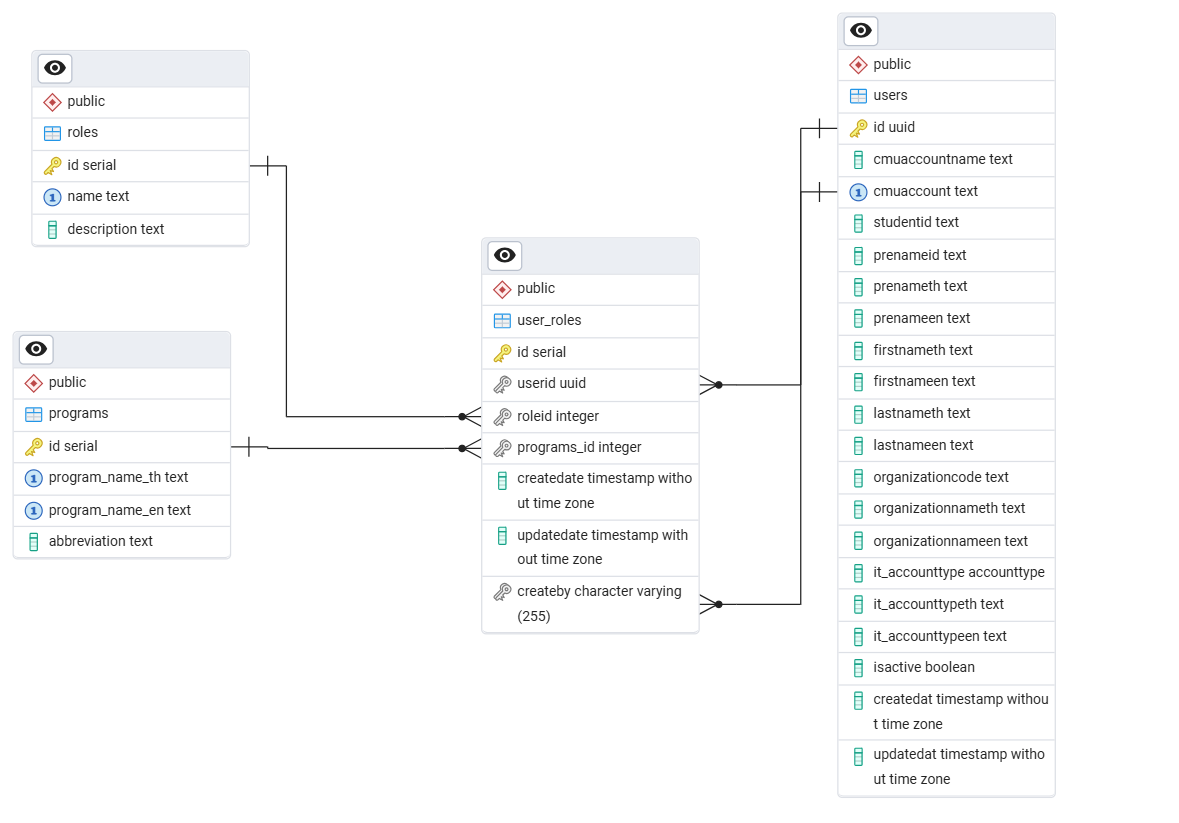
\includegraphics[width=0.8\textwidth]{pictures/auth_db.png}
  \caption{รูปภาพแสดง Database Schema ของ Auth Service}
  \label{fig:auth_service}
\end{figure}
\textbf{\ifenglish Database Schema\else โครงสร้างของฐานข้อมูล\fi}
\begin{itemize}
  \item \textbf{users} ตารางนี้จะเป็นตารางที่เก็บข้อมูลของผู้ใช้งาน 
  \item \textbf{roles} ตารางนี้จะเป็นตารางที่เก็บข้อมูลของตำแหน่งของผู้ใช้งาน
  \item \textbf{programs} ตารางนี้จะเป็นตารางที่เก็บข้อมูลของโปรแกรมหรือหลักศสูตรที่มีอยู่ในระบบ
  \item \textbf{user\_roles} ตารางนี้จะแสดงถึงความสัมพันธ์ของผู้ใช้งานกับตำแหน่งของผู้ใช้งานในโปรแกรมหรือหลักสูตรนั้นๆ
\end{itemize}
\subsection{Project Service}
\subsection{Search Service}

\chapter{\ifproject%
\ifcpe การทดลองและผลลัพธ์\else Experimentation and Results\fi
\else%
\ifcpe การประเมินระบบ\else System Evaluation\fi
\fi}

ในบทนี้จะทดสอบเกี่ยวกับการทำงานในฟังก์ชันหลักๆ

\ifproject
\chapter{\ifenglish Conclusions and Discussions\else บทสรุปและข้อเสนอแนะ\fi}

\section{\ifenglish Conclusions\else สรุปผล\fi}

\hspace{1.27cm}ในบทนี้จะสรุปถึงข้อจำกัดของระบบในด้านต่างๆ ที่ระบบมีในเนื้อหาส่วนนี้ด้วย
\begin{itemize}
  \item ระบบสามารถรวบรวมและจัดเก็บข้อมูลโปรเจกต์จบของนักศึกษาได้อย่างมีประสิทธิภาพ
  \item ผู้ใช้สามารถค้นหาและเข้าถึงข้อมูลโปรเจกต์ได้ง่ายขึ้น
  \item ระบบมีการจัดการสิทธิ์การเข้าถึงข้อมูลที่ดี ทำให้ข้อมูลมีความปลอดภัย
  \item อย่างไรก็ตาม ระบบยังมีข้อจำกัดในด้านการแสดงผลบนอุปกรณ์มือถือ และการจัดการข้อมูลที่มีขนาดใหญ่
\end{itemize}

\section{\ifenglish Challenges\else ปัญหาที่พบและแนวทางการแก้ไข\fi}

\hspace{1.27cm}ในการทำโครงงานนี้ พบว่าเกิดปัญหาหลักๆ ดังนี้
\begin{itemize}
  \item การจัดการข้อมูลที่มีขนาดใหญ่และการค้นหาข้อมูลที่มีประสิทธิภาพยังคงเป็นปัญหา
  \item การแสดงผลบนอุปกรณ์มือถือยังไม่รองรับอย่างเต็มที่
  \item การค้นหาข้อมูลจากในโครงงานยังไม่สามารถแสดงผลได้ว่าอยู่ส่วนไหนของโครงงาน
\end{itemize}

\section{\ifenglish Suggestions and further improvements\else ข้อเสนอแนะและแนวทางการพัฒนาต่อ\fi}

\hspace{1.27cm}ข้อเสนอแนะเพื่อพัฒนาโครงงานนี้ต่อไป มีดังนี้
\begin{itemize}
  \item ปรับปรุงการแสดงผลให้รองรับการใช้งานบนอุปกรณ์มือถือ
  \item พัฒนาระบบการจัดการข้อมูลให้มีประสิทธิภาพมากขึ้น โดยใช้เทคโนโลยีการจัดการข้อมูลที่เหมาะสม
  \item ปรับปรุงการจัดการสิทธิ์การเข้าถึงข้อมูลให้ใช้งานง่ายและมีความปลอดภัยมากขึ้น
  \item เพิ่มฟีเจอร์การค้นหาข้อมูลที่มีประสิทธิภาพและรวดเร็ว เช่นการเพิ่มการค้นหาจาก keyword
\end{itemize}
\fi

\bibliography{sampleReport}

\ifproject
\appendix
\chapter{The first appendix}

Text for the first appendix goes here.

\section{Appendix section}

Text for a section in the first appendix goes here.

test ทดสอบฟอนต์ serif

\textsf{test ทดสอบฟอนต์ sans serif}

\ifenglish\else
% TODO: Thai teletype font still doesn't work with english option
\verb+test ทดสอบฟอนต์ teletype ภาษาไทย+

\texttt{test ทดสอบฟอนต์ teletype ภาษาไทย}
\fi

\chapter{\ifenglish Manual\else คู่มือการใช้งานระบบ\fi}

Manual goes here.


%% Display glossary (optional) -- need glossary option.
\ifglossary\glossarypage\fi

%% Display index (optional) -- need idx option.
\ifindex\indexpage\fi

\begin{biosketch}
\begin{center}
  
\includegraphics[width=1.5in]{mugshot.jpg}
\end{center}
Your biosketch goes here. Make sure it sits inside
the \texttt{biosketch} environment.
\end{biosketch}
\fi % \ifproject
\end{document}
